\documentclass{article}
\usepackage[T1]{fontenc}
\usepackage{lmodern}
\usepackage{graphicx}
\usepackage{amsmath,amssymb}
\usepackage[a4paper,margin=2cm]{geometry}
\usepackage[absolute,overlay]{textpos}
\setlength{\TPHorizModule}{1mm}
\setlength{\TPVertModule}{1mm}
\usepackage[indonesian]{babel}
\usepackage{hyperref}
\setlength{\emergencystretch}{2em}
% unit: Halaman 31

\begin{document}

% === Halaman 31 (llm) ===

Dekripsi:

\vspace{60mm}

\begin{align*}
R_{i-1} &= L_i \\
L_{i-1} &= R_i \oplus f(R_{i-1}, K_i) = R_i \oplus f(L_i, K_i)
\end{align*}

% deskripsi: Diagram alur proses dekripsi Feistel cipher yang menunjukkan hubungan antara L, R, fungsi f, dan kunci K.
% bbox normalisasi: [0.1300, 0.1900, 0.8400, 0.7900]
\begin{textblock*}{149.10mm}(27.30mm,56.43mm)
\noindent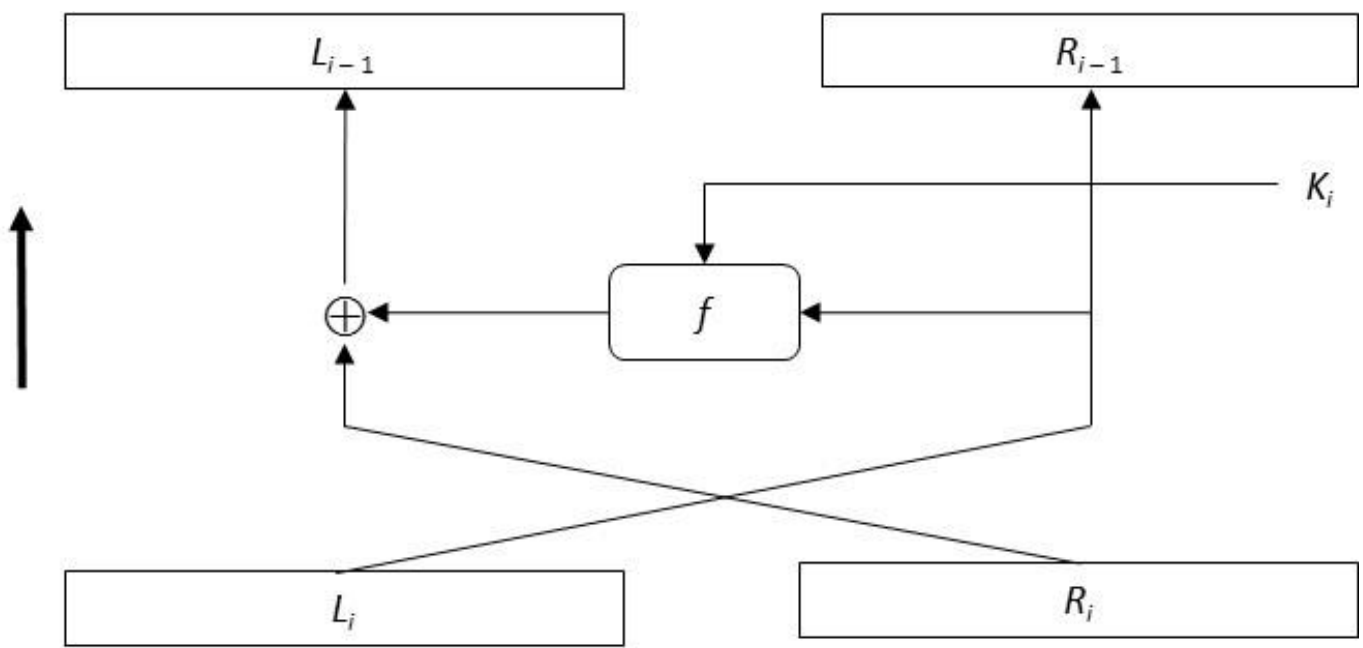
\includegraphics[width=149.10mm,height=178.20mm]{../../images/llm/page_031_img_01.png}%
\end{textblock*}

\end{document}
